\chapter{Déroulement factuel du stage}
\clearpage

\section{Prise de fonction et intégration}
À l'arrivée au sein de l'\ac{ARCOP}, l'intégration s'est effectuée au sein de la Direction des Statistiques et de la Documentation. Une présentation de l'organisation et des missions du service a permis de mieux comprendre son fonctionnement. Les objectifs du stage ainsi que les attentes du tuteur ont ensuite été exposés.
Durant cette phase d'intégration, plusieurs actions ont été réalisées :

\begin{itemize}
    \item Découvert l'environnement de travail et les outils utilisés.
    \item Pris en main les méthodologies internes et les processus en place.
    \item Échangé avec les membres de l'équipe pour mieux comprendre les besoins et le cadre du stage.
\end{itemize}

\section{Tâches effectuées}
Tout au long du stage à la Direction des Statistiques et de la Documentation de l'\ac{ARCOP}, plusieurs tâches ont été effectuées, notamment:
\begin{itemize}
    \item Développement de projets applicatifs (OptiHR et Gestion des Recours)
    \item Installation et maintenance des équipements informatiques
    \item Débogage du réseau téléphonique IP de l'entreprise 
    \item Support aux utilisateurs de la \ac{PASSE}
    \item Assistance technique générale    
\end{itemize} 

\subsection{Développement de projets applicatifs}

\subsubsection{Projet OptiHR : Digitalisation des processus RH}

\paragraph{Découverte du projet et études préliminaires}
L'un des objectifs principaux de mon stage était la \textbf{digitalisation des processus de travail du département des \ac{RH}}. Avant d'entamer le développement, plusieurs tâches préparatoires ont été réalisées :

\begin{itemize}
    \item Analyse des besoins du département en collaboration avec le responsable du département des \ac{RH}.
    \item Étude des solutions existantes et identification des axes d'amélioration.
    \item Participation aux réunions pour recueillir les attentes des utilisateurs.
    \item Rédaction d'un cahier des charges et validation des fonctionnalités essentielles avec mon tuteur.
\end{itemize}

\paragraph{Développement de la solution numérique}
Après cette phase d'étude, j'ai entamé la conception et le développement de l'application. Cela a inclus :
\begin{itemize}
    \item La mise en place de l'environnement de développement (choix des technologies, configuration des outils).
    \item La conception de l'architecture du projet et de la base de données.
    \item Le développement des premières fonctionnalités, notamment \textbf{l'authentification et la gestion des utilisateurs}.
    \item Des tests et des ajustements basés sur les retours du tuteur et des futurs utilisateurs.
\end{itemize}

Par la suite, d'autres fonctionnalités ont été intégrées, comme :

\begin{itemize}
    \item La gestion des documents administratifs.
    \item L'automatisation de certaines tâches du département des \ac{RH}.
    \item L'amélioration de l'interface utilisateur pour une meilleure expérience.
\end{itemize}

\paragraph{Finalisation du projet et restitution}
Dans les dernières semaines du stage, mon travail s'est concentré sur :

\begin{itemize}
    \item La finalisation du développement et la correction des derniers bugs.
    \item La rédaction de la documentation technique et utilisateur.
    \item La présentation du projet aux responsables du département des \ac{RH} et la collecte des feedbacks.
    \item La formation des collaborateurs à l'utilisation de la solution développée.
\end{itemize}

\subsubsection{Projet Gestion des Recours}

\paragraph{Contexte et objectifs}
En parallèle du projet OptiHR, j'ai été impliqué dans le développement d'un système de gestion des recours pour optimiser le suivi et le traitement des contestations liées aux marchés publics. Ce projet visait à améliorer l'efficacité du processus de traitement des recours et à faciliter leur suivi par les différents acteurs concernés.

\paragraph{Analyse des besoins et conception}
Cette phase a comporté plusieurs activités essentielles :
\begin{itemize}
    \item Organisation de réunions avec la Direction des Affaires Juridiques pour comprendre précisément le processus de gestion des recours.
    \item Analyse du flux de travail actuel et identification des points d'amélioration.
    \item Élaboration des spécifications fonctionnelles en collaboration avec les utilisateurs clés.
    \item Conception de l'architecture de la solution en tenant compte des contraintes techniques et organisationnelles.
\end{itemize}

\paragraph{Développement de l'application}
Le développement de la solution de Gestion des Recours a été réalisé en plusieurs étapes :
\begin{itemize}
    \item Création de la structure de base de données pour stocker les informations relatives aux recours.
    \item Développement du module d'enregistrement des recours, permettant de saisir les informations essentielles (requérant, autorité contractante, date de dépôt, objet).
    \item Implémentation du système de suivi des différentes étapes de traitement des recours.
    \item Mise en place des fonctionnalités de filtrage avancé (par date, par décision, par requérant, etc.).
    \item Développement du module de visualisation graphique pour l'analyse statistique des recours.
    \item Intégration d'un système de notifications automatiques pour alerter sur les recours en attente de traitement.
\end{itemize}

\paragraph{Tests et mise en production}
La phase finale du projet a consisté en :
\begin{itemize}
    \item Tests approfondis avec les utilisateurs finaux pour valider l'adéquation de la solution aux besoins.
    \item Ajustements et corrections des anomalies identifiées lors des tests.
    \item Migration des données existantes vers le nouveau système.
    \item Formation des utilisateurs à l'utilisation de l'application.
    \item Déploiement progressif de la solution dans l'environnement de production.
\end{itemize}

\paragraph{Résultats et bénéfices}
Le système de Gestion des Recours a permis d'obtenir plusieurs améliorations significatives :
\begin{itemize}
    \item Réduction du temps de traitement des recours grâce à une meilleure organisation du flux de travail.
    \item Amélioration de la transparence du processus pour toutes les parties concernées.
    \item Disponibilité d'indicateurs de performance clairs pour le suivi de l'activité.
    \item Accès facilité aux archives des recours précédents pour établir des précédents et assurer la cohérence des décisions.
\end{itemize}

\subsection{Installation et maintenance des équipements informatiques}
Cette mission a consisté à assurer le bon fonctionnement du matériel informatique en effectuant :
\begin{itemize}
    \item L'installation et la configuration des ordinateurs de bureau pour les employés.
    \item La mise en place et la mise à jour des logiciels antivirus afin de garantir la sécurité des données.
    \item Le diagnostic et la résolution des pannes matérielles et logicielles.
\end{itemize}

\subsection{Débogage du réseau téléphonique IP de l'entreprise}
Afin d'assurer le bon fonctionnement des communications internes, une intervention sur le réseau téléphonique IP a été menée :
\begin{itemize}
    \item Analyse des dysfonctionnements et identification des causes des interruptions de service.
    \item Participation aux interventions techniques visant à rétablir la connexion et la qualité des appels.
    \item Assistance aux utilisateurs pour résoudre les problèmes liés à la téléphonie IP.
\end{itemize}

\subsection{Support aux utilisateurs de la \acs{PASSE}}

\subsubsection{Présentation de la PASSE}
La \textbf{\ac{PASSE}} (\textit{Plateforme de l'ARCOP pour des Services Sécurisés et Électroniques}) est un outil numérique conçu pour optimiser la gestion et le suivi des services économiques. Elle permet aux opérateurs économiques d'effectuer diverses démarches administratives en ligne et d'accéder aux informations essentielles liées à leurs activités, notamment la demande d'attestation de régularité de la taxe parafiscale.

La plateforme est accessible via le lien suivant :  
\url{https://passe.arcop.tg}  

\subsubsection{Accompagnement des utilisateurs}
Afin d'assurer une utilisation optimale de la plateforme et garantir une expérience fluide aux opérateurs économiques, un dispositif de support et d'assistance technique a été mis en place :

\begin{itemize}
    \item \textbf{Participation au comité de suivi de la \ac{PASSE}} : Contribution active aux échanges et décisions visant à améliorer le fonctionnement et l'efficacité de la plateforme.
    
    \item \textbf{Assistance technique} : Un accompagnement personnalisé est proposé aux opérateurs économiques, notamment pour l'accès à la plateforme, la soumission des documents et l'utilisation des différents services en ligne.
\end{itemize}

\subsubsection{Captures d'écran}
Pour mieux illustrer l'interface et les principales fonctionnalités de la \ac{PASSE}, voici quelques captures d'écran :

\begin{figure}[H]
    \centering
    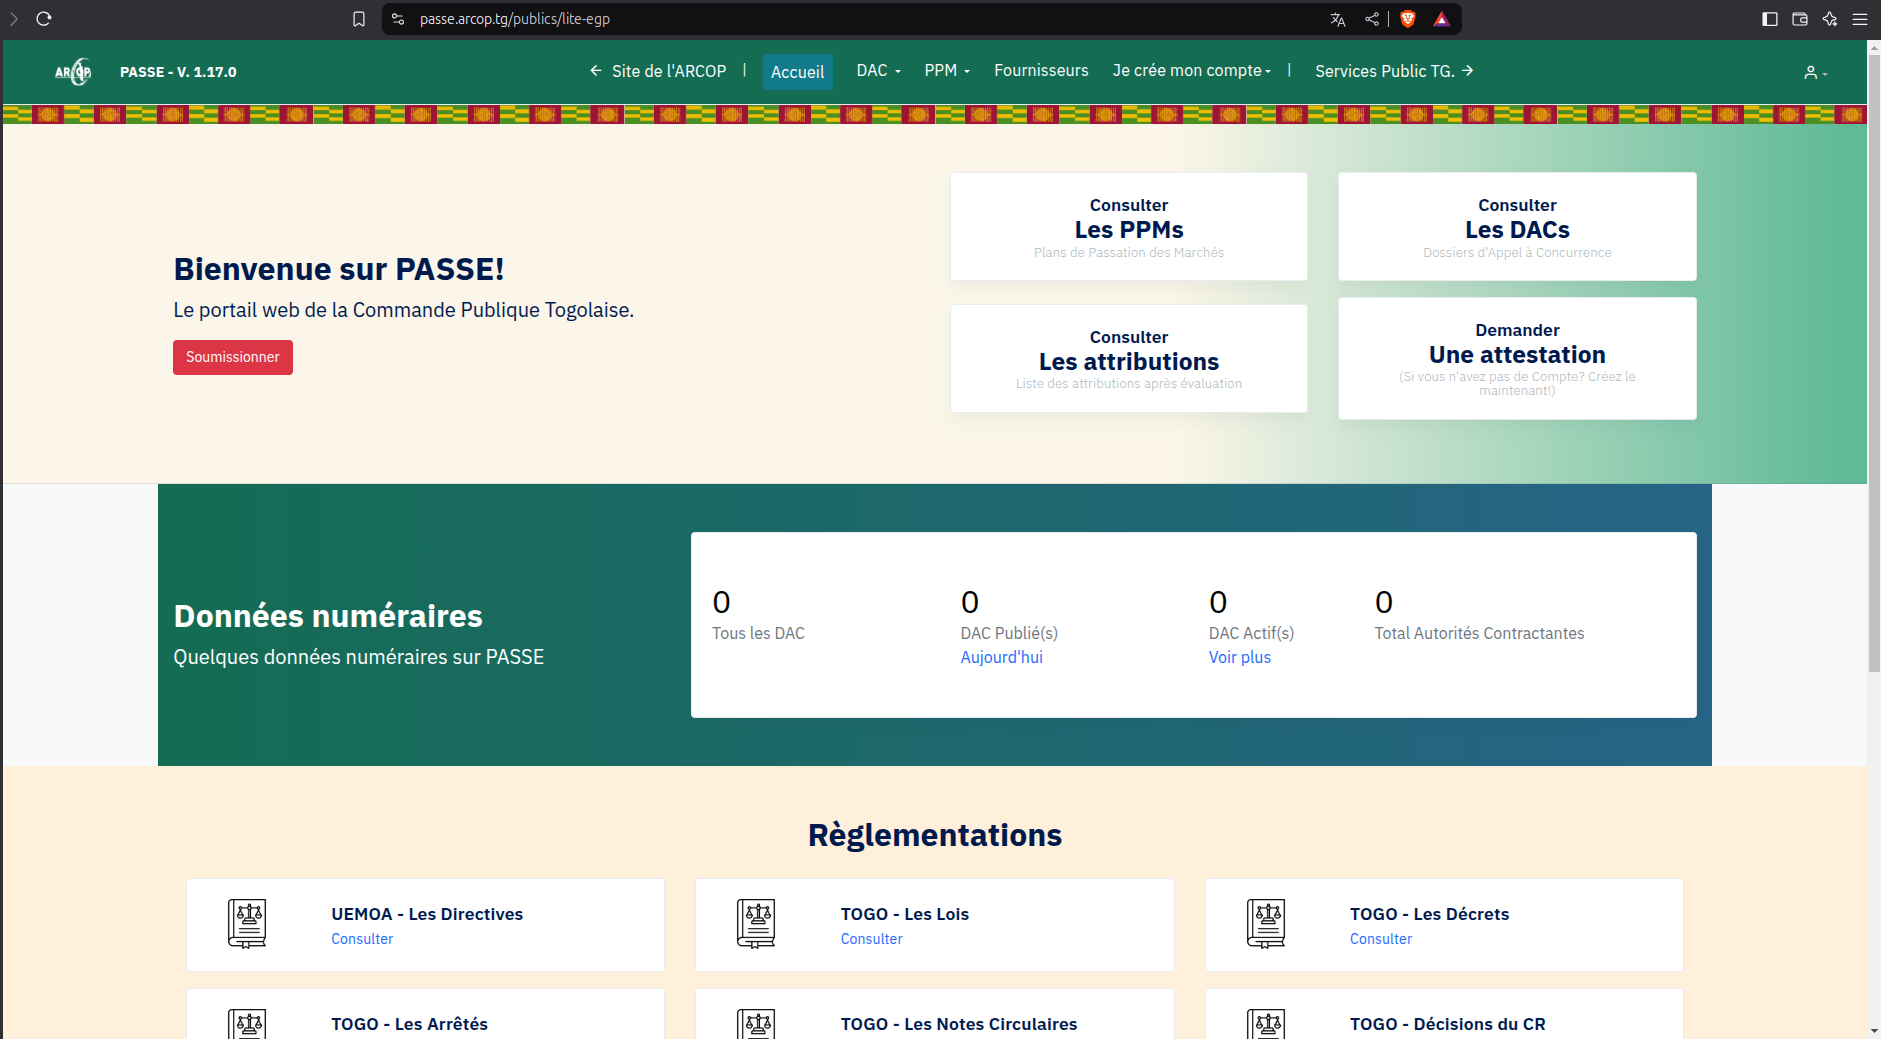
\includegraphics[width=0.8\textwidth]{images/passe/home.png}
    \caption{Page d'accueil de la \ac{PASSE}}
    \label{fig:page-accueil_pass}
\end{figure}

\begin{figure}[H]
    \centering
    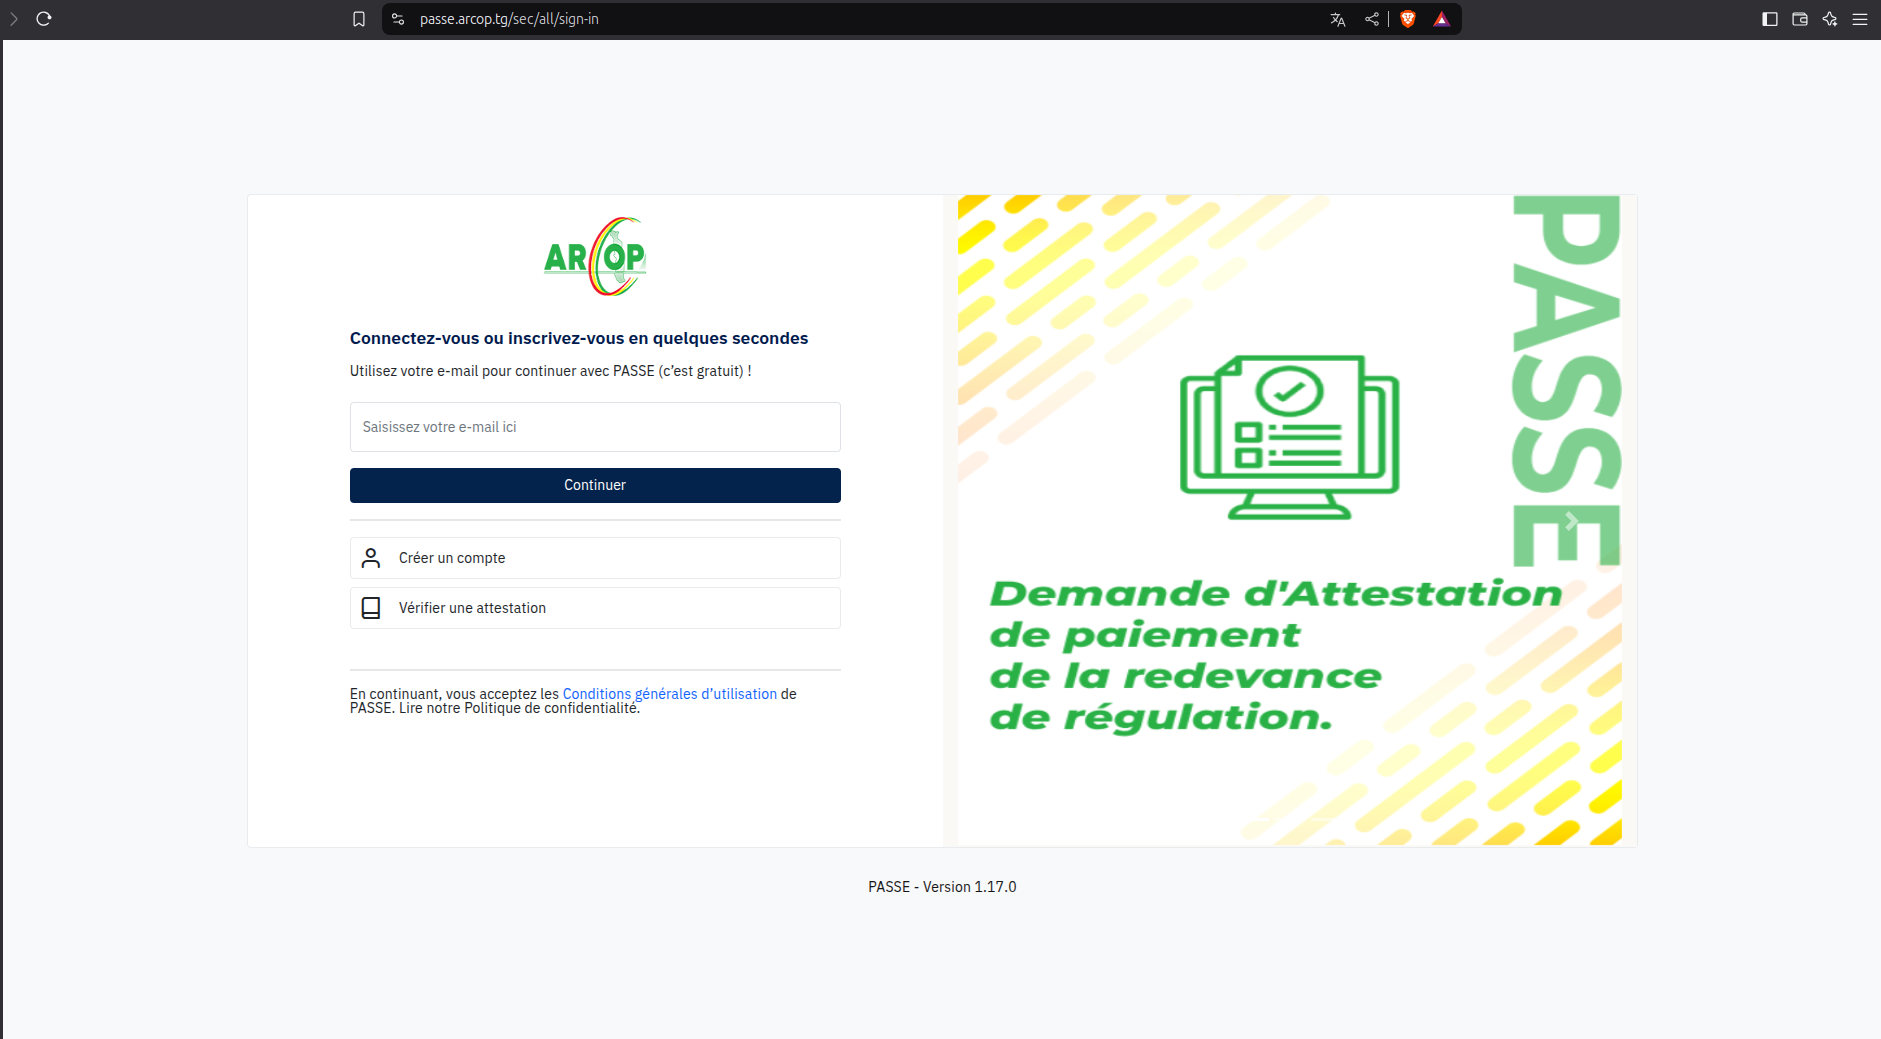
\includegraphics[width=0.8\textwidth]{images/passe/login.png}
    \caption{Interface de connexion de la \ac{PASSE}}
    \label{fig:interface-login_pass}
\end{figure}

\subsection{Assistance technique générale}
En complément des missions spécifiques, un support technique global a été assuré au sein de l'organisation :
\begin{itemize}
    \item Dépannage et maintenance des outils informatiques utilisés par le personnel.
    \item Configuration et optimisation des postes de travail selon les besoins des employés.
    \item Sensibilisation aux bonnes pratiques pour garantir la pérennité des équipements et la sécurité des données.
\end{itemize}

\section{Remarques et suggestions}

Au terme de ce stage au sein de la Direction des Statistiques et de la Documentation de l'ARCOP, plusieurs observations et recommandations peuvent être formulées dans une perspective d'amélioration continue.

\subsection{Concernant les projets de développement}

\begin{itemize}
    \item \textbf{Intégration des systèmes} : Il serait bénéfique d'envisager une intégration plus poussée entre les différentes applications développées au sein de l'ARCOP (OptiHR, Gestion des Recours, PASSE) afin de créer un écosystème numérique cohérent.
    
    \item \textbf{Méthodologie de développement} : L'adoption d'une méthodologie agile plus formalisée permettrait d'améliorer le suivi des projets et d'impliquer davantage les utilisateurs tout au long du cycle de développement.
    
    \item \textbf{Documentation technique} : La mise en place d'un système de documentation technique centralisé faciliterait la maintenance et l'évolution des applications développées.
\end{itemize}

\subsection{Concernant l'infrastructure informatique}

\begin{itemize}
    \item \textbf{Renouvellement planifié du parc informatique} : Certains équipements atteignent leur limite d'âge et nécessiteraient un plan de renouvellement progressif pour éviter les interruptions de service.
    
    \item \textbf{Consolidation de la sécurité informatique} : La mise en place d'une politique de sécurité plus robuste, incluant des formations régulières pour les utilisateurs, permettrait de réduire les risques liés aux cybermenaces.
    
    \item \textbf{Optimisation du réseau téléphonique IP} : Suite aux interventions effectuées, il serait judicieux d'investir dans une solution plus stable et moderne pour garantir la fiabilité des communications internes.
\end{itemize}

\subsection{À propos de la Plateforme PASSE}

\begin{itemize}
    \item \textbf{Amélioration de l'expérience utilisateur} : L'interface de la PASSE gagnerait à être simplifiée pour les opérateurs économiques moins familiers avec les outils numériques.
    
    \item \textbf{Documentation utilisateur enrichie} : La création de guides détaillés et de tutoriels vidéo permettrait de réduire le nombre de sollicitations auprès du support technique.
    
    \item \textbf{Mise en place d'un système de feedback} : L'intégration d'un mécanisme permettant aux utilisateurs de signaler les problèmes ou suggérer des améliorations contribuerait à l'évolution positive de la plateforme.
\end{itemize}

\subsection{Remarques générales}

\begin{itemize}
    \item \textbf{Standardisation des procédures} : L'élaboration de procédures standardisées pour la gestion des incidents informatiques optimiserait le temps de résolution et garantirait une qualité de service constante.
    
    \item \textbf{Veille technologique} : La mise en place d'une veille active sur les innovations technologiques pertinentes pour l'ARCOP permettrait d'anticiper les évolutions nécessaires.
\end{itemize}

Ces suggestions s'inscrivent dans une démarche d'amélioration continue visant à optimiser l'efficacité des processus et la qualité des services proposés par l'ARCOP, tant en interne qu'auprès des opérateurs économiques.

\section{Bilan et conclusion}
Cette expérience a permis de mieux appréhender les enjeux liés à la gestion d'un service informatique, alliant développement d'applications métier, assistance aux utilisateurs et maintenance technique. Les deux projets principaux, OptiHR et Gestion des Recours, ont contribué à la transformation numérique de l'ARCOP en optimisant des processus critiques pour l'organisation. Cette immersion professionnelle a également offert l'opportunité d'acquérir une vision globale des problématiques IT dans un contexte institutionnel.

\clearpage